\subsubsection{Tipos}
Hay tres tipos distintos de \acrshort{rnn}:
\begin{itemize}
    \item Muchos a uno: A partir de una secuencia generar un vector. Por ejemplo, valorar del uno al diez opiniones sobre productos escritas por clientes.
    \item Muchos a muchos: A partir de secuencia generar una secuencia. Por ejemplo, traducir texto de un idioma a otro.
    \item Uno a muchos: A partir de un solo vector se genera una secuencia. Por ejemplo, una red especializada en describir los elementos de una imagen.
\end{itemize}

\begin{figure}[H]
    \centering
    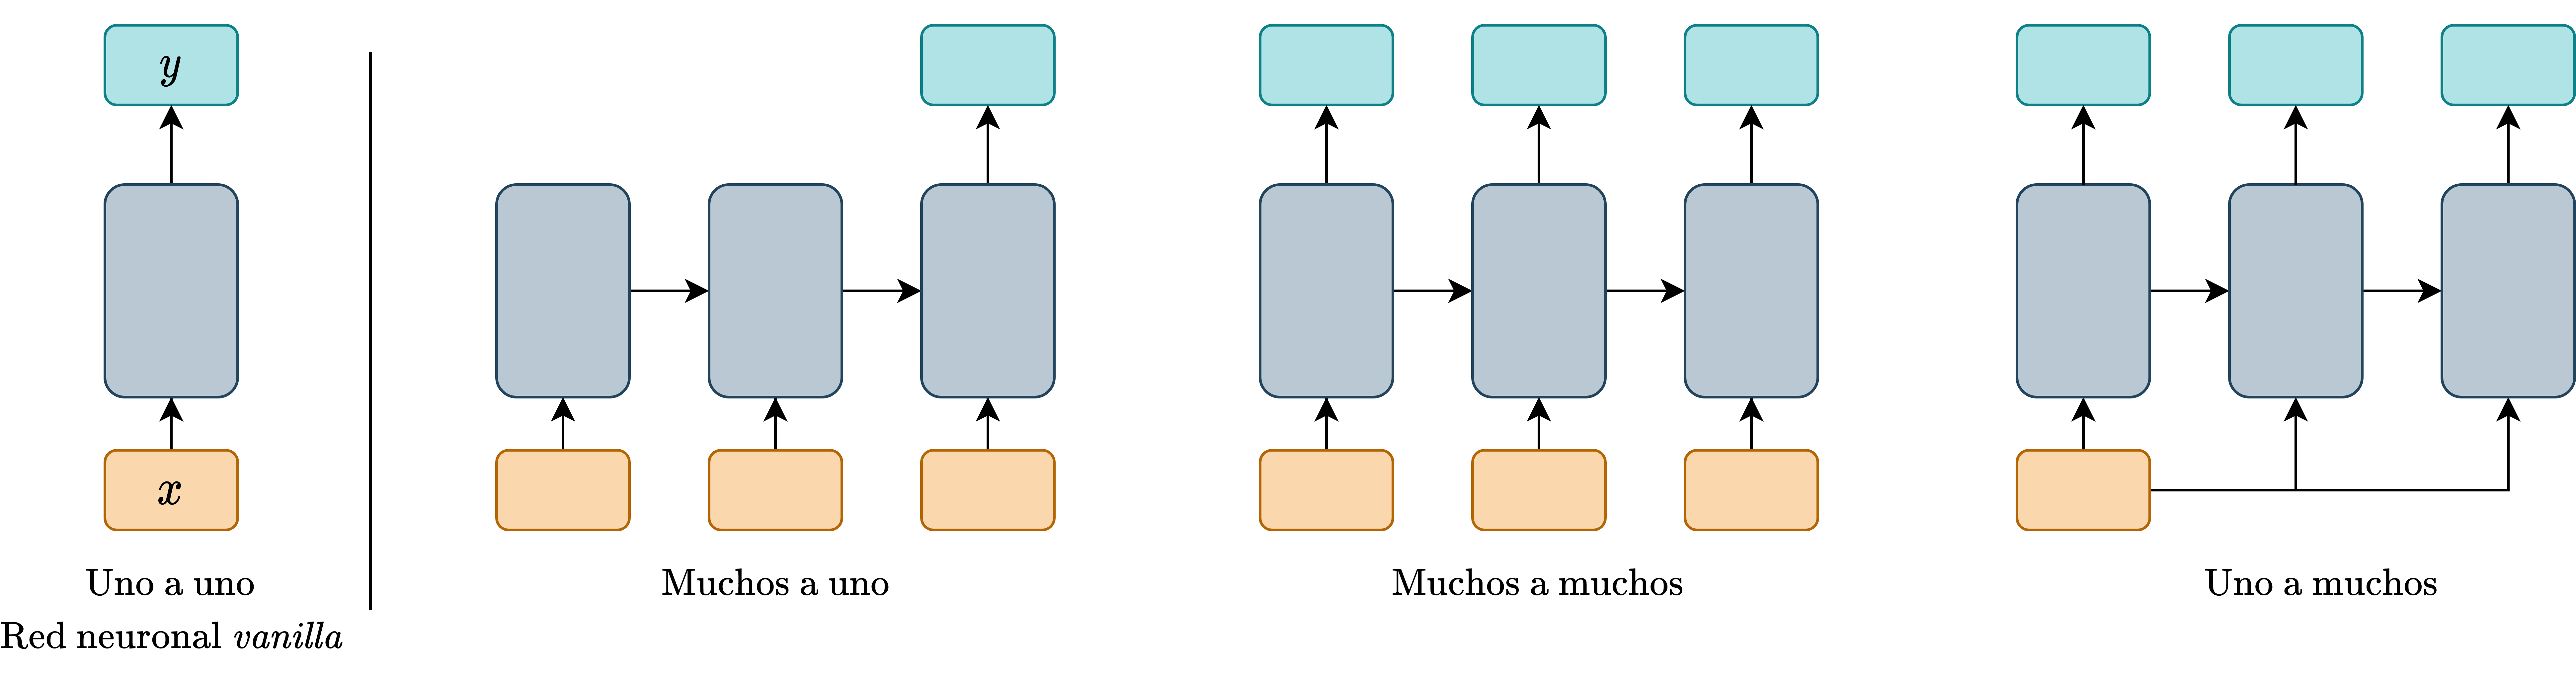
\includegraphics[width=14cm]{images/state-of-art/rnn/rnn-types.png}
    \caption{Representación de funcionamiento de los tipos de \acrshort{rnn}}
    \label{fig:rnn_types}
\end{figure}
